\documentclass[a4paper]{article}

\usepackage{amsmath, blindtext, float, graphicx, hyperref}
\graphicspath{ {./images/} }
\title{REAL: Retrieval-Augmented Language MOdel Pre-Training}
\author{Shubham Gupta}

\begin{document}
\maketitle
\section{Introduction}
\begin{itemize}
    \item REALM is a paper mentioned in the T5 paper titled: \textbf{How Much Knowledge Can You Pack Into The Parameters of a Language Model?}
    \item TLDR: This paper retrieves documents that have the information present while solving Question-Answer type problems.
    \item Introduced a latent \textit{knowledge retriever}, which can attend and retrieve documents over large corpus and can be trained in unsupervised manner using masked language modelling technique and backprop through retreiver which considers lots of docs.
        \begin{figure}[H]
            \centering
            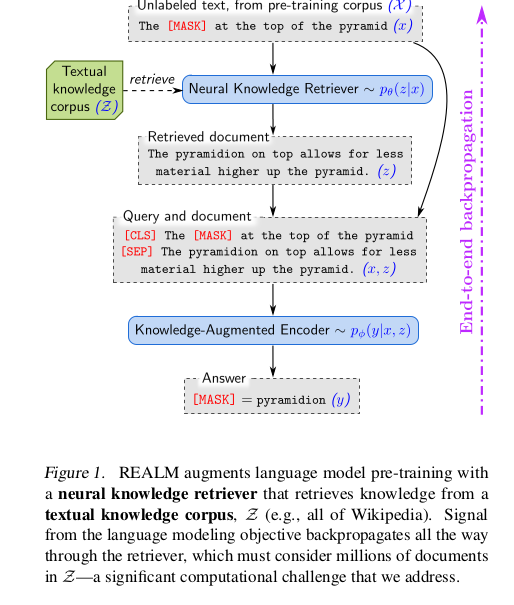
\includegraphics[width=0.8\textwidth]{training}
            \caption{Training process for REALM}
            \label{fig:training}
        \end{figure}
    \item Key point: Train retriever using a performance-based signal from unsupervised text.
    \item Retrieval based LM => Moar computational resources => Moar money
        \begin{itemize}
            \item Solution: Computation performed for each doc is cached and can be used again. Best doc selected using \textit{Maximum Inner Product Search(MIPS)}. Read the paper \href{https://cs.stanford.edu/~ermon/papers/ICML_MIPS_Gumbel.pdf}{here}.  
        \end{itemize}
    \item REALM retriever can be used on downstream tasks via transfer learning.
    \item REALM is SOTA on NQ-Open, WQ and CuratedTrec.
\end{itemize}
\section{Approach}
\subsection{\textit{Retreive-then-predict generative process} }
\begin{itemize}
    \item Training: Masked-LM. Fine-tuning: Open QA task
    \item $p(y|x)$ decomposed into two steps:
        \begin{itemize}
            \item Given $x$,retrive documents $z$ from corpus $Z$. Modelled as: $p(z|x)$
            \item Condition of both $z$ and $x$ to generate output $y$ i.e p(y|z, x)
            \item Overall likelihood $y$ is generated by treating  $z$ as latent variable and marginalizing over all documents $z$ 
                \begin{equation}
                    \begin{split}
                        p(y|x) = \sum_{z \Inn Z} p(y|z, x) * p(z|x)
                    \end{split}
                \end{equation}
        \end{itemize}
\end{itemize}
\subsection{Architecture}
\begin{itemize}
    \item \textbf{Neural Knowledge Retriever} i.e models $p(z|x)$ 
    \item \textbf{Knowledge Augmented Encoder} i.e models p(y|z, x) 
\end{itemize}
\subsection{Neural Knowledge Retriever}
\begin{itemize}
    \item Dense inner product model.
        \begin{equation}
            \begin{split}
                p(z|x) = \frac{exp(f(x,z))}{\sum_{z^'} exp(f(x,z^')}
                \\ f(x,z) = Embed_{input}(x)^TEmbed_{doc}(z)
            \end{split}
        \end{equation}
    \item $Embed_{input}$ and $Embed_{doc}$ are embedding functions
    \item f(x,z) is called \textbf{relevance score}. It is inner product of vector embeddings. 
    \item Relevant Distribution is softmax over all relevance scores 
    \item Embedding implement using BERT-style transformers. Join using <SEP>, prefix using <CLS> and append <SEP> as the end.
        \begin{equation}
            \begin{split}
                \\ join_{BERT}(x) = [CLS]x[SEP]
                \\ join_{BERT}(x_1, x_2) = [CLS]x_1[SEP]x_2[SEP]
            \end{split}
        \end{equation}
    \item Pass above into transformer, which gives over vector for each token. Perform linear projection to reduce dimensionality of vector
        \begin{equation}
            \begin{split}
                \\ Embed_{input}(x) = W_{input}BERT_{CLS}(join_{BERT}(x))
                \\ Embed_{doc}(z) = W_{doc}BERT_{CLS}(join_{BERT}(z_{title}, z_{body}))
            \end{split}
        \end{equation}
\end{itemize}
\subsection{Knowledge-Augmented Encoder}
\begin{itemize}
    \item Given input  $x$ and relevant doc $z$, this defines  $p(y|z,x)$
    \item Join $x$ and $z$ into single sequence and feed into transformer
    \item Here, training is different for pre-training vs fine-tuning
    \begin{itemize}
        \item For pre-training, predict [MASK] token. Use same Masked LM(MLM) loss as in Transformer(Devlin)
        \item For Open-QA, we need to produce string $y$. Assumption: $y$ occurs as sequence of tokens in some document in the corpus. Skipping the math bit for now.
    \end{itemize}
\end{itemize}
\subsection{Training}
\begin{itemize}
    \item Compute gradients in $\theta$ and $\phi$ and optimize using SGD.
    \item Challenge: Computing $p(y|x)$
    \item Approx by summing over top $k$ documents with highest prob under $p(z|x)$
    \item Question: How to find top $k$ docs? Answer: Use MIPS
    \item Need to precompute $Embed_{doc}(x)$ for all docs. Problems? It changes with each step of SGD.
    \item \textit{Solution}: Async refresh $Embed_{doc}$ every 500 steps
    \item Use MIPS to select top $k$ docs. For these docs, recompute $p(z|x)$ using new $\theta$.
\end{itemize}
\end{document}
